\documentclass[a4paper,12pt]{article}

\usepackage[spanish]{babel}
\usepackage[utf8]{inputenc}
\usepackage[T1]{fontenc}
\usepackage[utf8]{inputenc}
\usepackage{makeidx}
\usepackage{graphicx}
\usepackage{lmodern}
\usepackage{kpfonts}
\usepackage[left=2cm,right=2cm,top=2cm,bottom=2cm]{geometry}
\usepackage{amsmath,amsfonts,amssymb}
\usepackage{setspace}

\title{Parcial 1}
\author{Junior Miguel Lara Torres}
\date{today}

\graphicspath {{C:/Users/JuniorLara/Desktop/TexMaker_Files/}}
\begin{document}

\begin{center}
\par 
\includegraphics[scale=1]{USB} \par
Universidad Simon Bolivar \\ Curso: CI2613 / Algoritmos y Estructuras III \\ Trimestre: Septiembre-Diciembre, 2022 \\ Profesor: Wilmer Bandres \\ Estudiante: Junior Miguel Lara Torres - Carnet: 17-10303 \\
\end{center}

\begin{center}
Parcial 1
\end{center}

\textbf{ * Repaso de conceptos (4 puntos)}

\begin{enumerate}

\item Diga la razón por la cual un grafo euleriano implica la existencia de un ciclo euleriano (1 pt).

\begin{flushleft}
Al tomar un nodo n random del grafo, empezamos una recorrido armando un camino C. Sabemos que cuando comenzamos en n usamos un arco para salir de él, sin embargo por definición de grafo euleriano todo nodo tiene grado par, por tanto en algún punto del camino debemos regresar a n. El razonamiento es que como existe grado par en cada nodo entonces tenemos salida y entrada para todo nodo, por tanto en algún punto para el camino que estamos armando se repetirá el nodo inicial. Con esto garantizamos que se forma un ciclo. Ahora falta probar que es un ciclo euleriano, es decir que se recorren todos los arcos.

Para esta segunda parte de la prueba, cuando tomemos un ciclo random mediante el argumento anterior sabemos que hemos usado una cantidad par de arcos. Por tanto, si consideramos esos nodos faltantes por arcos sin utilizar, aplicamos el mismo argumento y creamos un segundo ciclo, esto porque sabemos que todo nodo siempre tendrá salida y entrada. Entonces, al crear mas ciclos es sabido que todos están conectados y podemos concatenar los caminos y concluimos que existe un ciclo euleriano de todo el grafo. 

\end{flushleft}

\item De un ejemplo de una representación implícita de un grafo (1 pt).

\begin{flushleft}
* Existe un nodo por cada número natural (Sin el 0).\\
* Existe un arco entre dos $x,y \in V \iff div(x+y)=2$. Esto seria que existira una arista si la suma de los nodos conectados es un numero primo (Divisores de x+y es 2). Así, la representación como función es $f: V \times V \setminus \{\{x,x\}: \forall x \in V \} \to bool$ tal que $f(x,y) = |\{ \forall m \in \mathbb{N} \land m \leq \lfloor (x+y)/2 \rfloor : m|(x+y) \}| = 1$. 

Es decir, considerar la mitad de los numeros posibles para una división entera, con obtener candinalidad 1 se tiene que m = 1 fue el único divisor, mas el número percé x+y que cuanta como divisor, entonces decimos que x+y es primo.
\end{flushleft}
$~~$ \\
$~~$ \\
$~~$ \\
$~~$ \\

\item Marque aquellas proposiciones que son verdaderas (2 pts).

\begin{flushleft}
Las proposiciones marcadas como ciertas son: (Están en el form igualmente)
\begin{itemize}
\item En un grafo no dirigido si un nodo x alcanza a un nodo y, entonces y también alcanza a x.

\item Remover un puente de un grafo conexo aumenta el número de componentes conexas

\item Un árbol con n nodos contiene n-1 puentes.

\item En la representación de un grafo mediante lista de adyacencias, agregar un nodo es una operación sin mucho costo
\end{itemize}

\end{flushleft}

\end{enumerate}

\textbf{ * Ejercicios prácticos (9 pts)}

\begin{enumerate}

\item Dé Ejemplos de un clique maximal y un clique máximo. Puede ser un dibujo (con PDF) o escrito con la notación de G=(V,E) (1 pt).

\begin{center}
\par 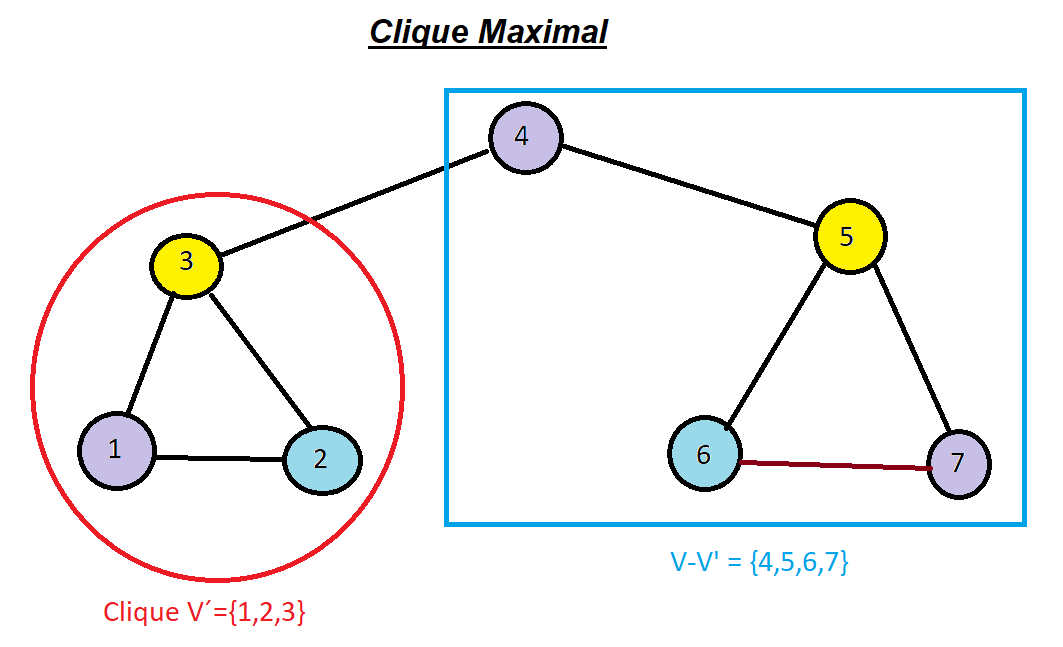
\includegraphics[scale=0.7]{p1} \par
\end{center} 

Notemos que al agregar el nodo 4 al clique éste deja de ser un grafo completo, lo que deja de ser un clique.

\begin{center}
\par 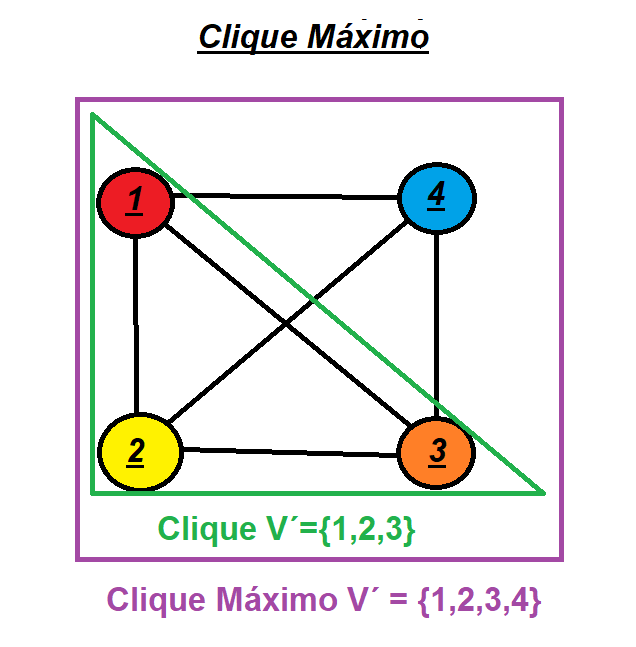
\includegraphics[scale=0.7]{p2} \par
\end{center} 

Veamos que el clique V' es uno de varios que se pueden formar, pero tenemos como máximo al formado por $\{1,2,3,4\}$.

\item Diga si el siguiente grafo es euleriano y encuentre un ciclo euleriano si lo es. Si no lo es explique por qué. (1 pt).

\begin{center}
\par 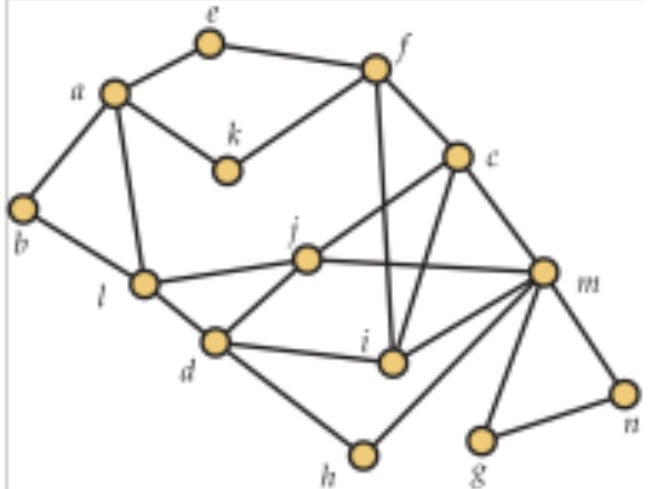
\includegraphics[scale=0.8]{im1} \par
\end{center} 

\begin{flushleft}
Dado que todo nodo x del grafo tiene grado par, entonces cumple con la definición de grafo euleriano. Para el ciclo euleriano la definicion dice que existe y el siguiente: 
$C = \langle j, c, m, n, g, m, h, d, i, m, j, d, l, b, a, e, f, c, i, f, k, a, l, j \rangle$
$~~$ \\
$~~$ \\
$~~$ \\
$~~$ \\
\end{flushleft}

\item De un ejemplo de un grafo dirigido que tenga por lo menos un circuito. Y luego dé su grafo reducido. Puede dibujarlo o simplemente usar las notaciones vistas en clases con G=(V,E) (2 pts).

\begin{flushleft}

\begin{center}
\par 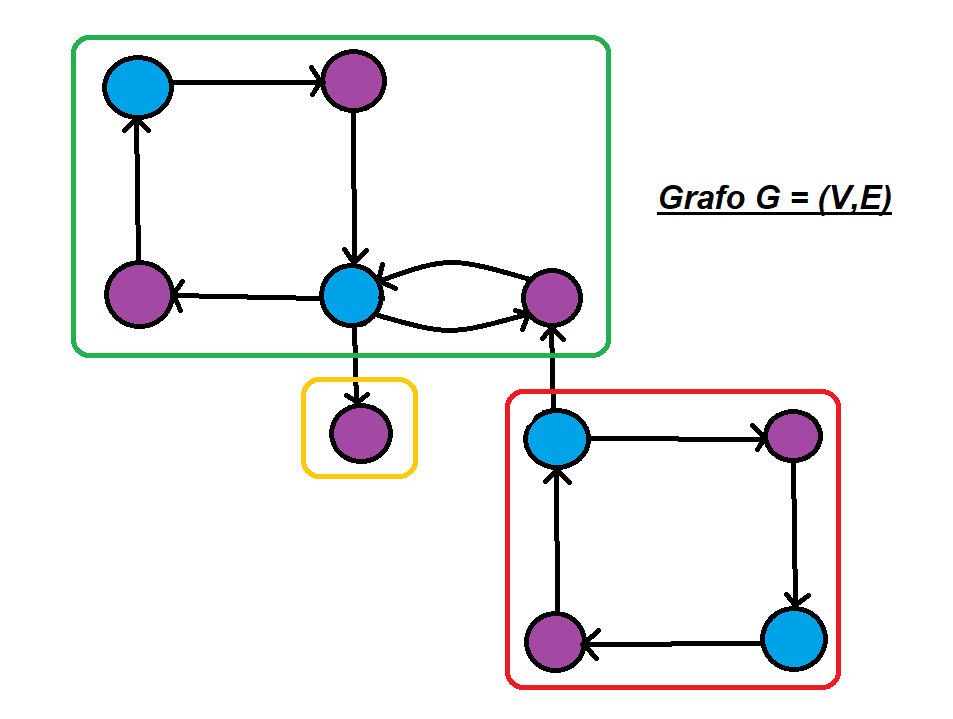
\includegraphics[scale=0.7]{p3} \par
\end{center}

\begin{center}
\par 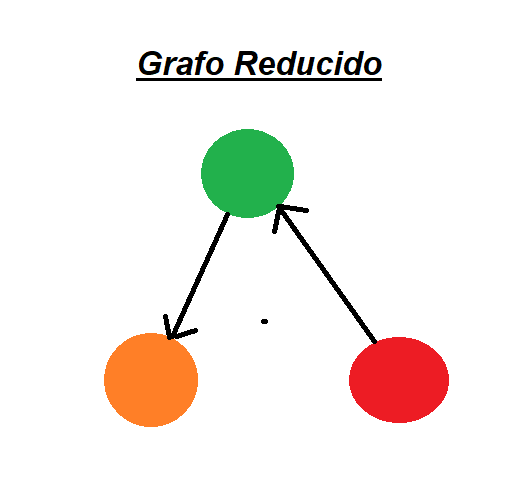
\includegraphics[scale=0.7]{p4} \par
\end{center}

\end{flushleft}

\item Dado un grafo (no dirigido) euleriano escriba un algoritmo para construir un ciclo euleriano (2 pts).

\begin{flushleft}

Se crea una función BuscarArco que dado el conjunto E y el nodo n ha buscar en él, cuando se encuentre se saca del conjunto y se retorna. Siempre se encontrará un arco para un nodo actual, es decir un nodo donde 'Estoy actualmente' pues esto simula como si hubiese 'llegado' al nodo por un camino y a no ser que sea el caso de concluir todas las aristas del grafo (terminar el ciclo) entonces existe un arco de salida. \\
$~~$ \\
Tupla BuscarArco(set E, int n) $\{$ \\
$~~~~~~$ Para $e \in E$ hacer $\{$ \\
$~~~~~~~~~~~~$ Si $n \in e \land $ hacer $\{$ \\
$~~~~~~~~~~~~~~~~~~$ arc $\leftarrow$ E.sacar(e);\\
$~~~~~~~~~~~~~~~~~~$ del $\leftarrow$ arc.sacar(n);\\
$~~~~~~~~~~~~~~~~~~$ return arc;\\
$~~~~~~~~~~~~$ $\}$ \\
$~~~~~~$ $\}$ \\
$\}$ \\
$~~$ \\
input: G = (V,E); \\
e $\leftarrow$ E.sacar(); \\
CE $\leftarrow \emptyset$; \\
CS $\leftarrow$ e.sacar(); \\
Mientras $E \neq \emptyset$ hacer $\{$ \\
$~~~~~~$ nActual = e.sacar();\\
$~~~~~~$ e $\leftarrow$ BuscarArco(E,nActual); \\
$~~~~~~$ CS $\leftarrow$ nActual; \\
$~~~~~~$ Si $CS.inicial() == CS.Final()$ hacer $\{$ \\
$~~~~~~~~~~~~$ CE $\leftarrow$ Concatenar(CE,CS); \\
$~~~~~~~~~~~~$ e $\leftarrow$ E.sacar(); \\
$~~~~~~~~~~~~$ CS $\leftarrow$ e.sacar(); \\
$~~~~~~$ $\}$ \\
$\}$ \\
$~~$ \\
Agregamos al ciclo CS los nodos que vamos recorriendo, cuando este CS tenga como nodo inicial igual al final entonces se formó un ciclo y se debe concatenar con CE. \\
$~~$ \\
Supongamos que existe una función para los conjuntos set.sacar() que retorna un elemento random y elimina el elemento y set.sacar(x) retorna el elemento x del conjunto y lo elimina del set. \\
$~~$ \\
La función concatenar para un ejemplo digamos que, $CE = \langle 1, 2, 1 \rangle$ y $Cs = \langle 2, 3, 2 \rangle$, entonces el resultado es $CE = \langle 1, 2, 3, 2, 1 \rangle$.
\end{flushleft}

\item Dado un tablero de ajedrez como el mostrado en la imagen. Imagínese que quitamos la esquina superior derecha y la esquina inferior izquierda. Ahora imagínese que empezamos a cubrir el tablero con piezas de domino, donde una pieza cubre exactamente 2 cuadritos contiguos. 
Diga un argumento mediante grafos de por qué es imposible cubrir todo el tablero con piezas de domino sin que ninguna pieza sobresalga del tablero. (3 pts)

\begin{center}
\par 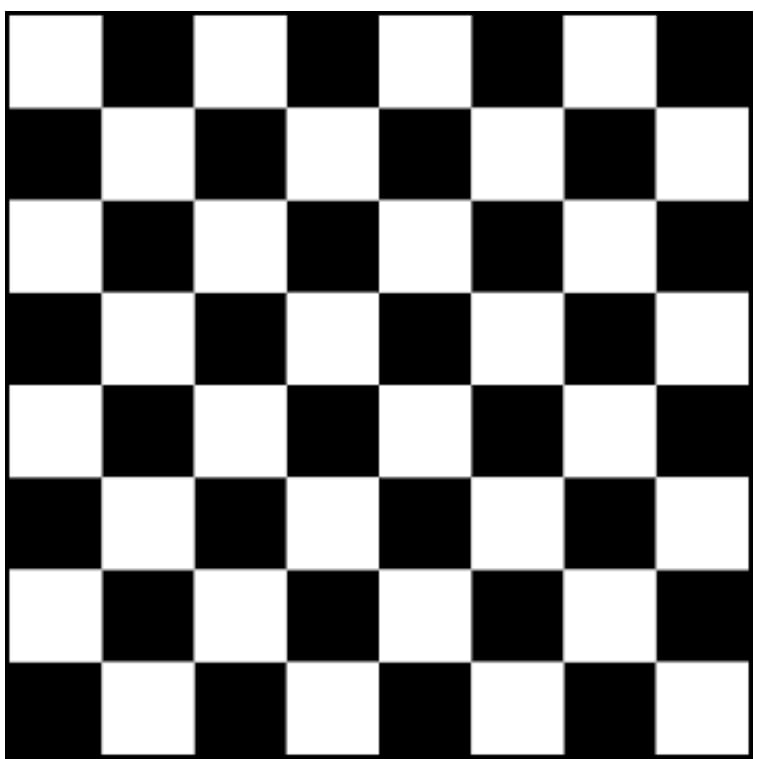
\includegraphics[scale=0.8]{im2} \par
\end{center}

\begin{flushleft}

\end{flushleft}
La analogía planteada es que cada cuadro en la fila/columna es una conexión con otra fila/columna, por tanto al quitar el cuadro superior derecho e inferior izquierdo se esta cortando una conexión con otra la fila/columna, es decir pasar de tener una conexión par (8 cuadros) a impar (7 cuadros), esto sucede en puntos extremos, por tanto es como simular un grafo semi-euleriano donde exactamente dos nodos tiene grado impar y los demás tienen grado par. Recordemos que por teorema no existe un ciclo euleriano sino un camino euleriano que empieza y termina en distintos nodos, ambos términos se relacionan con poder y no poder llenar el tablero. \\
$~~$ \\
En otros términos, veamos que cuando se hace la acción de colocar una ficha de domino ocurren dos casos, se coloca vertical entonces estamos pasando a nivel de filas de un nodo a otro, si se coloca horizontal estamos pasando de una columna a otra, esto lo interpretamos como recorrer los nodos pero en concreto pasamos de color negro a color blanco o viceversa. Ahora se tiene una cantidad inequivalente de zonas, tenemos 32 zonas blancas y 30 zonas negras a pesar de quitar 2 cuadros de los 64, esto nos permite concretar que se deben 30 caminos de 31 que necesitábamos a nivel de grafo. Así, determinamos una noción de que no es posible finalizar un camino en el mismo nodo de comienzo, lo que genera un grafo semi-euleriano o visto de otra forma todo 'nodo blanco' conecta con un 'nodo negro', pero como tenemos 30 en un grupo y 32 en otro, solo usamos 30 dominós/arcos lo que deja 2 'cuadros/nodos blancos' sin conexión lo que finalmente decir que no es posible llenar el tablero. 

\end{enumerate}
 $~~$ \\
 $~~$ \\
 \textbf{ * Demuestre o dé un contraejemplo para las siguientes proposiciones. En caso de dar un contraejemplo explíquelo (12 puntos)}

\begin{enumerate}

\item Un grafo euleriano no puede tener un ciclo hamiltoniano (2 pt).

\begin{flushleft}

\begin{center}
\par 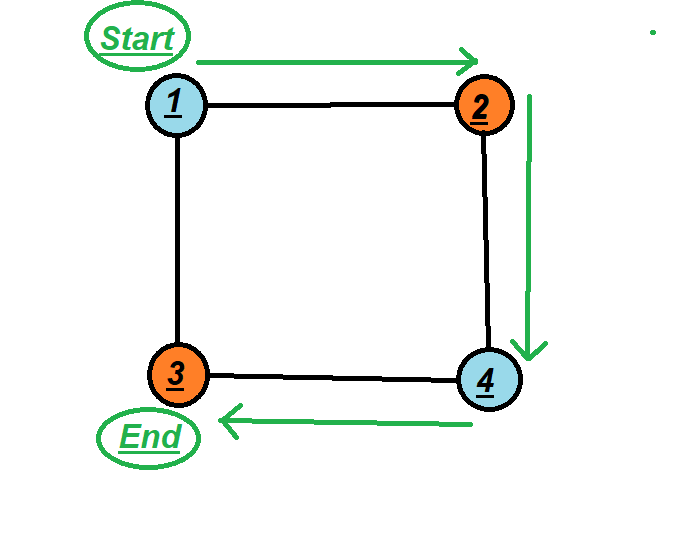
\includegraphics[scale=0.8]{p5} \par
\end{center}

Vemos que el grafo mostrado todo nodo tiene grado par lo que se define como grafo euleriano y a su vez vemos el camino hamiltoniano $C = \langle 1,2,4,3 \rangle$.

\end{flushleft}

\item Un árbol es un grafo conexo con exactamente n-1 arcos, donde n es el número de nodos del grafo. Note que un árbol no tiene ciclos.
Proposición: El número cromático de un árbol es 2. (3 pts).

\begin{flushleft}
Veamos que si analizamos los niveles de un árbol, podemos tomar los niveles pares e impares, como también podemos analizar los hijos de un nodo padre. Recordando que un árbol tiene un nodo raíz, empezando el argumento desde allí, los hijos es sabido que no tienen conexión entre ellos (aristas) por tanto los hijos de la raíz tienen todos el mismo color que es diferente al del padre, así mismo analizamos los hijos de los hijos, ellos no tienen conexión directa con el abuelo, por tanto pueden tener el color del abuelo, realizando este argumento para cada nivel del árbol, obtenemos dos subconjuntos para colorear con 2 colores distintos ambos, por tanto el numero cromático de un árbol es 2.
\end{flushleft}

\item En un grafo con n nodos, todo camino simple tiene menos de n arcos (3 pts).

\begin{flushleft}
Por definición de camino simple es aquel que no repite nodos. Ahora, como se considera a todo tipo de grafos (En un grafo con n nodos, ...) podemos considerar el grafo de $n \geq 1$ nodos donde existan algún/algunos nodos con grado 0 pero por definición de camino elemental es el camino con un solo nodo, lo que claramente es menor que los n arcos. Por otra parte, tener en el peor de los grafos un camino que pase por todos los n nodos y en un camino se sabe que empieza y termina en un nodo diferente, de lo contrario serie un ciclo, por tanto tenemos que el camino tendrá menos de n arcos en el peor de los casos.

\end{flushleft}

\item Todo grafo conexo contiene un punto de articulación (2 pts).

\begin{flushleft}

\begin{center}
\par 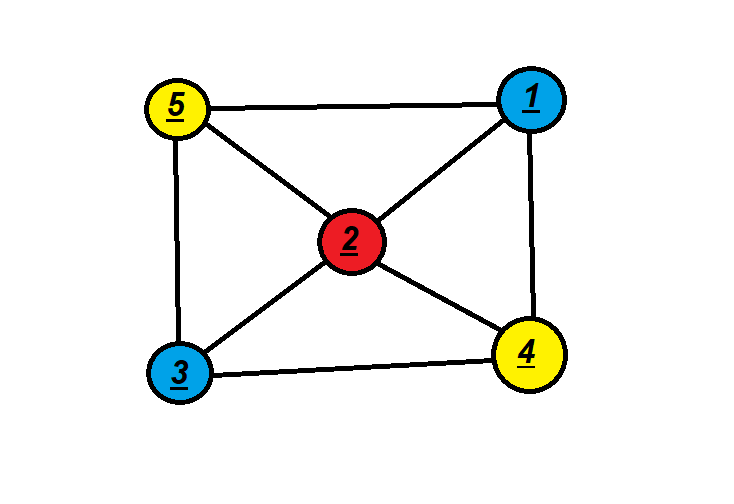
\includegraphics[scale=0.8]{p6} \par
\end{center}

Este contraejemplo prueba que no importa que nodo quite seguirá conexo pues para todo par de nodos existe un camino. \\

\end{flushleft}

\item Dado que un grafo contiene un grafo bipartito completo de n+m nodos donde n es el número de nodos en uno de los dos conjuntos disjuntos de nodos del grafo bipartito y m el número de nodos en el otro conjunto. Dado que n >= 1 y m >= 1 entonces el número cromático del grafo es por lo menos min(n,m) + 1. (2 pts).

\begin{flushleft}

\begin{center}
\par 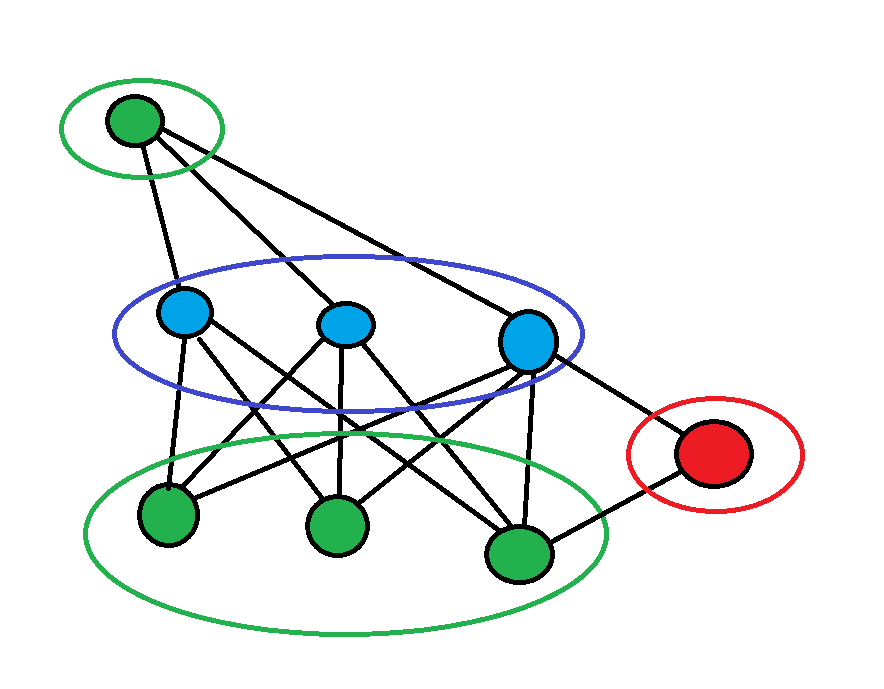
\includegraphics[scale=0.8]{p7} \par
\end{center}

\end{flushleft}

Notemos que el conjunto verde tiene n=4 elementos, el conjunto azul tiene m=3 elementos, por tanto min(n,m)+ 1 = 3 + 1 = 4. Es decir que el numero cromático debe ser 4, pero notemos que es posible colorear con 3 colores el grafo dado.

\end{enumerate}

\textbf{ * Puntos extra (4 puntos)}

\begin{enumerate}

\item CodeForces 1

\begin{flushleft}

\end{flushleft}

\item CodeForces 2

\begin{flushleft}

\end{flushleft}

\end{enumerate}
 
\end{document}